\documentclass{article}
\usepackage{graphicx} % Required for inserting images
\usepackage{courier} %% Sets font for listing as Courier.
\usepackage{listings, xcolor}
\usepackage{exercise}

\usepackage{mathtools}
\usepackage{amssymb}
\usepackage{amsfonts}
\usepackage{graphicx}
\usepackage{float}
\usepackage{listings}
\usepackage{hyperref}
\usepackage{attachfile2}
\usepackage{vhistory}
\usepackage{epsfig}
\usepackage{subfig}
\usepackage{tikz}
\usetikzlibrary{external}
\tikzexternalize[prefix=tikz/]

\renewcommand\ExerciseName{Question~}
\renewcommand\AnswerName{Answer to question}
\renewcommand\ExerciseHeader{%
  \noindent\parbox[t]{.18\textwidth}{%
    \bfseries\large\ExerciseName\ExerciseHeaderNB\hfill}%
  \parbox[t]{.72\textwidth}{%
    \centering\bfseries\large%
    \ExerciseHeaderTitle\ExerciseHeaderOrigin}%
  \par\medskip
}

\newcommand{\addimg}[4]{
    \begin{figure}[H]
        \centering
        \includegraphics[#2]{#1}
    \caption{#3}
    \label{#4}
    \end{figure}
}

\lstset{
tabsize = 4, %% set tab space width
showstringspaces = false, %% prevent space marking in strings, string is defined as the text that is generally printed directly to the console
numbers = left, %% display line numbers on the left
commentstyle = \color{green}, %% set comment color
keywordstyle = \color{blue}, %% set keyword color
stringstyle = \color{red}, %% set string color
rulecolor = \color{black}, %% set frame color to avoid being affected by text color
basicstyle = \small \ttfamily , %% set listing font and size
breaklines = true, %% enable line breaking
numberstyle = \tiny,
}

\title{Language And Translators - TP Correction}
\author{Francesco Nieri}
\date{June 2024}

\begin{document}
\maketitle
\tableofcontents
\newpage
\section{TP1}
    \subsection{Question 1}
    
        Consider this piece of code from a fictional C-like programming language:
        \begin{lstlisting}[language = Java , frame = trBL , firstnumber = last , escapeinside={(*@}{@*)}]                 
int x2 = 25;
while(x2>0) {
    // increment x2 by one
    x2++;
    int y = fread(file) % 10;
    if(y<=4) {
        x2 = x2 - 1;
    }
    printf("Value: %d", y);
}
        \end{lstlisting}
        
        \subsubsection{Question 1.1}
    
            \textbf{Give the symbol classes that a lexer would need to lex this code (in the course, we have seen
            some basic classes, like Identifier, or Number). Also make symbol classes for whitespaces
            (space, newline), and comments.} \\
            
            
    We will combine question 1 and 3 together, the item on the left is the symbol class, on the right we have the regular expression.
\begin{itemize}
    \item Type: \texttt{int} 
    \item Space: \texttt{$\backslash$w } 
    \item Identifier: \texttt{$[a-zA-Z][azA-Z0-9]^{*}$}
    \item Assignment op: =
    \item Number: $[0-9]^{+}$
    \item String: " .* "
    \item Special char: [$;()\{\}$]
    \item Keyword: (if$|$while)
    \item Comparison operator: [$>|\le$]
    \item Increment operator: ++
    \item Comment : // .*$\backslash$n
    \item Math operator: ($-|\%$)
    \item EOL character: ;
    \item Param separator: ,
\end{itemize}
            
        \subsubsection{Question 1.2}
            \textbf{Write the sequence of symbols ($<$Token,Attribute$>$) that a lexer would generate for this code.} \\
            
            \begin{lstlisting}[language = bash , frame = trBL , firstnumber = last , escapeinside={(*@}{@*)}]
<Type, int > 
<Identifier, x2 > 
<Assignment operator, = >  
<Number, 25 >  
<EOL character, \backslashn >  
<Keyword, while>  
<Special character, ( > 
<Identifier, x2> 
<Comparison operator, > > 
<Number, 0 >  
<Special character, ) > 
<Special character, \{ > 
<Comment, //...> 
<Identifier, x2>     
<Increment operator, ++> 
<EOL character, ;> 
<Type, int> 
<Identifier, y> 
<Assignment operator, => 
<Identifier, fread> 
<Special character, (> 
<Math operator, \%> 
<EOL character, ;> 
<Keyword, if > 
<Special character, (> 
<Identifier, y> 
<Comparison operator, \le> 
<Number, 4> 
<Special character, )> 
<Special character, \{> 
<Identifier, x2> 
<Assignment operator, => 
<Identifier, x2> 
<Math operator, -> 
<Number, 1> 
<EOL character, ;> 
<Special character, \}> 
<Identifier, printf> 
<Special character, (> 
<String, "Value: \%d"> 
<Param separator, ,> 
<Identifier, y> 
<Special character, )> 
<EOL character, ;>   
<Special character, \}> 
\end{lstlisting}
            
    \subsection{Question 2}

        \subsubsection{Question 2.1}
        \textbf{The language of a RE can be described in English words. For example, one could say that the
        RE $(0|1)^{*}1$ stands for “all binary numbers ending with a 1”. Describe the RE} 
        \begin{center}
            $(0|1)^{*}0(0|1)^{*}0(0|1)^{*}$
        \end{center}
        \textbf{in English words.} \\
        
        Any binary sequence that contains at least two zeros
        
        \subsubsection{Question 2.2}
        \textbf{Construct a RE for “all binary numbers starting with a 1 and containing exactly one pair of
        consecutive 0”.} \\
        \begin{center}
            $1 (01|1)^{*}00(1|10)^{*}$
        \end{center}

    \subsection{Question 3}
        \subsubsection{Question 3.1}
            \textbf{Draw the NFA for RE $a(bc)^{*}(d|ef)$
            Indicate which state is the initial state and which states are the final states. See the NFA in
            question 3.5 on how to indicate the initial state and final states in an NFA diagram.}

            \addimg{img/TP1/3_1.pdf}{}{NFA for $a(bc)^{*}(d|ef)$}{}
            
        \subsubsection{Question 3.2}
            \textbf{Draw the NFA for $(a|b|bc)^{*}a$ and construct the DFA. The + sign can be used to express that a pattern must appear at least one time. What would be the NFA for the RE $(a|b|bc)^{+}a$ ?}
            
            \begin{figure}%
                \centering
                \subfloat[\centering]{{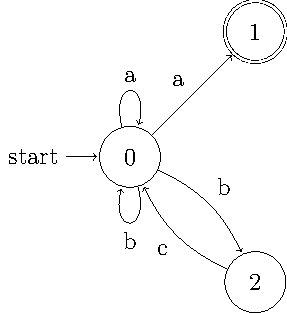
\includegraphics[width=5cm]{img/TP1/3_2a.pdf} }}%
                \qquad
                \subfloat[\centering ]{{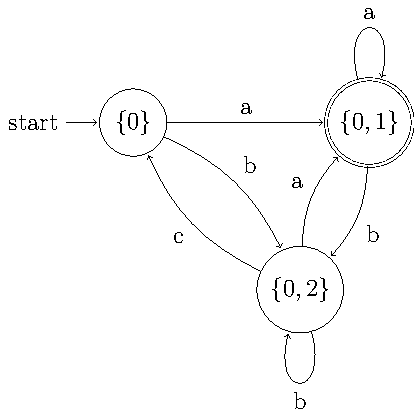
\includegraphics[width=5cm]{img/TP1/3_2b.pdf} }}%
                \caption{NFA and DFA for $(a|b|bc)^{*}a$}%
                \label{fig:example}%
            \end{figure}
           
            \addimg{img/TP1/3_2c.pdf}{}{NFA for $(a|b|bc)^{+}a$}{}

        \subsubsection{Question 3.3}
            \textbf{$\varepsilon$-transitions are very convenient if you want to combine two NFAs. Draw first the NFAs for $a^{*}$b and $c^{*}$d and then draw an NFA for ($a^{*}$b) $|$ ($c^{*}$ d) using $\varepsilon$-transitions.}

              \begin{figure}%
                \centering
                \subfloat[\centering]{{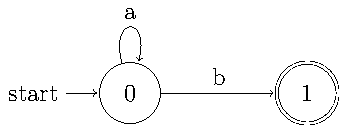
\includegraphics[width=5cm]{img/TP1/3_3a.pdf} }}%
                \qquad
                \subfloat[\centering ]{{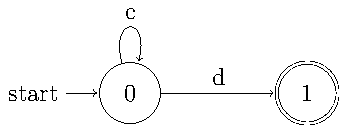
\includegraphics[width=5cm]{img/TP1/3_3b.pdf} }}%
                \caption{NFA and DFA for $(a|b|bc)^{*}a$}%
                \label{fig:example}%
            \end{figure}

           
            \addimg{img/TP1/3_3c.pdf}{}{NFA for ($a^{*}$b) $|$ ($c^{*}$ d)}{}

        \subsubsection{Question 3.4}
            \textbf{Transform the NFA for (a$^{*}$b) $|$ ($c^{*}$d) from question 3.3 into an NFA without $\varepsilon$-transitions.}

            \addimg{img/TP1/3_4.pdf}{}{NFA for (a$^{*}$b) $|$ ($c^{*}$d) without $\varepsilon$-transitions}{}

        \subsubsection{Question 3.5}
            \textbf{When dealing with NFAs with $\varepsilon$-transitions, it is useful to think about the $\varepsilon$-closure $\varepsilon$(s) of a state s, which is defined as the set of states that can be reached from that state s by doing one or several (!) $\varepsilon$-transition steps. For the below NFA over the alphabet $\Omega$ = {0,1}, give the $\varepsilon$-closures $\varepsilon$(A), $\varepsilon$(B), $\varepsilon$(C) of the states A, B, C.}

            \addimg{img/TP1/image.png}{width=0.5\textwidth}{}{}
        
            
$\varepsilon$-closures: 
\begin{center}
    \noindent $\varepsilon\{A\} = \{A, B, C\}$ \\
    $\varepsilon\{B\} = \{B, C\}$ \\
    $\varepsilon\{C\} = \{C\}$ \\
\end{center}
            \addimg{img/TP1/3_5.pdf}{}{DFA for the above graph}{}
        
        \subsubsection{Question 3.6}

            \textbf{Here is a modification of the powerset construction method seen in the course that also works with NFAs containing $\varepsilon$-transitions: \\
                • The initial state of the powerset automaton is $\varepsilon$({s0}). \\
                • The set of transitions T' of the powerset automaton is defined as:
                $\forall Q \subseteq S, c \in \Omega: (Q, c, R) \in T' for R = \varepsilon(\{t | s \in Q, (s, c, t) \in T)$
                Compare this modified method with the method that we have seen in the course. What is
                the difference?
                Transform the NFAs from question 3.3 (the combined NFA) and from question 3.5 into DFAs
                using this modified powerset construction method.}
    
            \addimg{img/TP1/3_6.pdf}{}{Combined DFA from NFAs}{}
\newpage
\section{TP2}
    \subsection{Question 1}
    \textbf{Consider the CFG G with the rules:}
    \begin{center}
        $S \rightarrow a \ | \ (S) \ | \ S \cdot S \ | \ S + S \ | \ -S $
    \end{center}
    \subsubsection{Question 1.1}
        \textbf{Give the set of terminal symbols used in the rules of G} \\

        \begin{center}
            $\Sigma = \{a, (, ), -, \cdot, +\}$
        \end{center}
    \subsubsection{Question 1.2}
        \textbf{Give a leftmost analysis of the input $a \cdot (-a + (a))$ and draw the syntax tree.} \\

        \noindent $(a \cdot (-a +(a)), S, \varepsilon)$ \\
$(a \cdot (-a +(a)), S \cdot S, 3)$ Rule 3 to expand S \\
$(a \cdot (-a +(a)), a \cdot S, 31)$ Rule 1 to expand S \\
$(\cdot (-a +(a)), \cdot S, 31)$ Match a \\
$( (-a +(a)), S, 31)$ Match $\cdot$ \\
$( (-a +(a)), (S), 321)$ Rule 2 to expand S \\
$( -a +(a)), S), 312)$ Match ( \\
$((-a +(a)), S + S), 3124)$ Rule 4 to expand S \\
$(-a +(a)), -S + S), 31245)$ Rule 5 to expand S \\
$( a +(a)), S + S), 31245)$ Match -\\
$( a +(a)), a + S), 312451)$ Rule 1 to expand S\\
$( +(a)),  + S), 312451)$ Match a\\
$( (a)),  S), 312451)$ Match +\\
$( (a)),  (S)), 3124512)$ Rule 2 to expand S\\
$( a)),  S)), 3124512)$ Match (\\
$( a)),  a)), 31245121)$ Rule 1 to expand S\\
$( )),  )), 31245121)$ Match a\\
$( ),  ), 31245121)$ Match )\\
$( \varepsilon,  \varepsilon, 31245121)$ Match )\\



        \addimg{img/TP2/1_2a.pdf}{}{Syntax tree for $a \cdot (-a + (a))$}{}
    \subsubsection{Question 1.3}
        \textbf{Give a rightmost analysis of the input $a \cdot (-a + (a))$}

        \noindent $(a \cdot (-a + (a)), S, \varepsilon)$ \\
$(a \cdot (-a + (a)), S \cdot S, 3)$ Rule 3 to expand S \\
$(a \cdot (-a + (a)), S \cdot (S), 32)$ Rule 2 to expand S \\
$(a \cdot (-a + (a)), S \cdot (S, 32)$ Match )  \\
$(a \cdot (-a + (a), S \cdot (S+S, 324)$ Rule 4 to expand S \\
$(a \cdot (-a + (a), S \cdot (S+S, 324)$ Rule 4 to expand S \\
$(a \cdot (-a + (a), S \cdot (S+(S), 3242)$ Rule 2 to expand S \\
$(a \cdot (-a + (a, S \cdot (S+(S, 3242)$ Match ) \\
$(a \cdot (-a + (a, S \cdot (S+(a, 32421)$ Rule 1 to expand S \\
$(a \cdot (-a + (, S \cdot (S+(, 32421)$ Match a \\
$(a \cdot (-a + , S \cdot (S+, 32421)$ Match ( \\
$(a \cdot (-a , S \cdot (S, 32421)$ Match + \\
$(a \cdot (-a , S \cdot (-S, 324215)$ Rule 5 to expand S \\
$(a \cdot (-a , S \cdot (-a, 3242151)$ Rule 1 to expand S \\
$(a \cdot (- , S \cdot (-, 3242151)$ Match a \\
$(a \cdot ( , S \cdot (, 3242151)$ Match - \\
$(a \cdot  , S \cdot , 3242151)$ Match ( \\
$(a, S, 3242151)$ Match $\cdot$ \\
$(a, a, 32421511)$ Rule 1 to expand S \\
$(\varepsilon, \varepsilon, 32421511)$ Match a \\

    \subsubsection{Question 1.4}
        \textbf{Show that G is ambiguous.}

        \noindent
With a leftmost derivation we can do the following: 
\begin{center}
    $S \xrightarrow{5} -S \xrightarrow{4} -S+S \xrightarrow{1} -a+S \xrightarrow{1} -a+a$ = \texttt{5411}. \\
\end{center}
But also: 
\begin{center}
    $S \xrightarrow{4} S+S \xrightarrow{5} -S+S \xrightarrow{1} -a+S \xrightarrow{1} -a+a$ = \texttt{4511}
\end{center}

\subsection{Question 2}
    \textbf{Extend the CFG for arithmetic expressions from the slides}

    \begin{center}
    $ E \rightarrow E + T \ | \ T$ \\
    $ T \rightarrow T \cdot F \ | \ F$ \\
    $ F \rightarrow (E) \ |\  Number \ | \ Identifier$
\end{center}

    \textbf{by:}

    \subsubsection{Question 2.1}
        \textbf{adding the binary minus operator and the division operator}

        \begin{center}
    $ E \rightarrow E + T \ | \  E - T \ | \ T$ \\
    $ T \rightarrow T \cdot F \ | \ T / F \ | \ F$ \\
    $ F \rightarrow (E) \ |\  Number \ | \ Identifier$
\end{center}

    \subsubsection{Question 2.2}
        \textbf{Write the syntax tree for 3 + 4/5. Then manually turn it into a more readable AST.}
            
            \begin{figure}[H]%
                \centering
                \subfloat[\centering]{{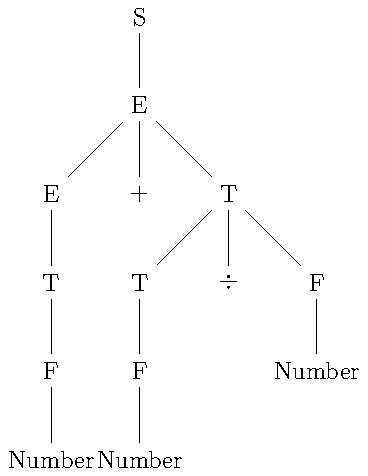
\includegraphics[width=5cm]{img/TP2/2_2a.pdf} }}%
                \qquad
                \subfloat[\centering ]{{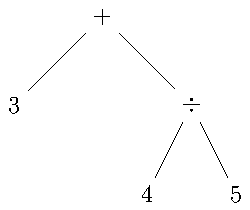
\includegraphics[width=5cm]{img/TP2/2_2b.pdf} }}%
                \caption{AST for 3 + 4/5 and readable AST}
                \label{fig:example}%
            \end{figure}

    \subsubsection{Question2.3}
        \textbf{You will notice that the AST in question 2 does not only reflect the syntactic structure of the
    input but also the precedence of the / operator over the + operator. Add a new operator $<$ to
    the grammar that has lower precedence than the + operator and the / operator and test the
    new grammar on the input $4+7 < 3 + 4/5.$}
    
    \begin{center}
    $ D \rightarrow D < E \ |\  E$ \\
    $ E \rightarrow E + T \ | \  E - T \ | \ T$ \\
    $ T \rightarrow T \cdot F \ | \ T / F \ | \ F$ \\
    $ F \rightarrow (E) \ |\  Number \ | \ Identifier$
\end{center}

    \addimg{img/TP2/2_3b.pdf}{}{}{}

\subsection{Question 3}
    \textbf{Here is a CFG for regular expressions over the alphabet {a, b}. That means the CFG describes how regular expressions look like.}

    \begin{center}
    $ S \rightarrow R $ \\
    $ R \rightarrow R + R \ | \  R R \ | \ R \cdot \ | T $ \\
    $ T \rightarrow (R)  | \ a \ | \ b$ \\
\end{center}

    \textbf{Note that we are using the plus-symbol “+” (e.g., “a+b”) to represent the choice in regular expression $(a|b)$ to avoid confusion with the $|$ used by the CFG itself. Run the NTA of this grammar for the input $a + (b \cdot)$}

    \noindent $(a + (b \cdot), S, \varepsilon)$ \\
$(a + (b \cdot), R, 1)$ Rule 1 to expand S \\
$(a + (b \cdot), R+R, 12)$ Rule 2 to expand S \\
$(a + (b \cdot), T+R, 125)$ Rule 5 to expand R \\
$(a + (b \cdot), a+R, 1257)$ Rule 7 to expand T \\
$( + (b \cdot), +R, 1257)$ Match a\\
$( (b \cdot), R, 1257)$ Match +\\
$( (b \cdot), T, 1257)$ Rule 5 to expand R\\
$( (b \cdot), (R), 125756)$ Rule 6 to expand T\\
$( b \cdot), R), 125756)$ Match (\\
$( b \cdot), R \cdot), 1257564)$ Rule 4 to expand R\\
$( b \cdot), T \cdot), 1257645)$ Rule 5 to expand R\\
$( b \cdot), b \cdot), 125767458)$ Rule 8 to expand R\\
$( \cdot), \cdot), 125767458)$ Match b\\
$( ), ), 125767458)$ Match $\cdot$\\
$( \varepsilon, \varepsilon, 125767458)$ Match )\\


\subsection{Question 4}
    \textbf{Consider the CFG G with the two rules}
    \begin{center}
        $S \rightarrow \ ab \ | \ ac$
    \end{center}
    \textbf{over the terminal symbols $\{a, b, c\}.$}

    \subsubsection{Question 4.1}
        \textbf{Explain why G is not LL(1). Is it LL(2) ?}

        \noindent A grammar is LL(1) if and only if, for all rules 
\begin{center}
    $A \rightarrow \beta | \gamma $ 
    
    $la(A \rightarrow \beta) \cap la(A \rightarrow \gamma) = \varnothing$
\end{center}
with $(\beta \ne \gamma)$  \\

\noindent It is not LL(1) as:
\begin{center}
    $first_{1}(S \rightarrow ab) = first_{1}(S \rightarrow ac) = \{a\}$
\end{center}

\noindent It is LL(2) as:
\begin{center}
    $first_{2}(S \rightarrow ab) = \{ab\} \ne first_{2}(S \rightarrow ac) = \{ac\}$
\end{center}

    \subsubsection{Question 4.2}
        \textbf{Write a CFG that is LL(1) and that generates the same language as G. Hint: the new grammar has two non-terminal symbols.}

        \begin{center}
    $S \rightarrow aR$ \\
    $R \rightarrow b \ | \ c$
\end{center}

    \subsubsection{Question 4.3}
        \textbf{Give a CFG similar to G that is not LL(5)}
        
        \begin{center}
    $S \rightarrow aaaaab \ | \ aaaaac$
\end{center}

\newpage
\section{TP3}
    \subsection{Question 1}
    \textbf{Show that any regular language can be generated by an LL(1) language.} \\
    
    For a regular language, we can write a regular grammar. That grammar corresponds to an NFA that
we can transform into a DFA. We will show that the DFA can be translated to a LL(1) grammar. 

Since a LL(1) grammar generates (or recognizes) a LL(1) language, we have achieved our goal.

To translate a DFA into an LL(1) grammar, we do the following:

The states of the DFA become non-terminal symbols and the transitions become terminal symbols in
the grammar.

Each transition in the DFA is translated to a rule in the grammar.

Example: the transition A $\xrightarrow{a}$ B of the DFA with two states A and B becomes the rule A $\rightarrow$ a B.

In the course, we have seen the theorem:
A grammar is LL(1) if and only if for all rules $A \rightarrow \beta | \gamma (\text{with} \beta \ne \gamma)$
$la(A \rightarrow \beta) \cap la(A \rightarrow \gamma) = \varnothing$
Having $la(A \rightarrow \beta) \cap la(A \rightarrow \gamma) \ne \varnothing$ is not possible in our case because that would mean that the
DFA had a state with two transitions with the same symbol, i.e., a non-deterministic transition.

\subsection{Question 2}
    \textbf{Consider the following grammar. This a CFG for regular expressions over the alphabet \{a, b\}}

    \begin{center}
    $S \rightarrow R$ \\
    $R \rightarrow R + T \ | \ R T \ | R \cdot \ | \ T$ \\
    $T \rightarrow (R) \ | \ a \ | \ b$ 
\end{center}
    \subsubsection{Question 2.1}
        \textbf{Transform the grammar into a grammar without left recursion and prove that the result is an LL(1) grammar.}

        \begin{center}
    $S \rightarrow R$  \\
    $R \rightarrow TR'$ \\
    $R' \rightarrow +TR' \ | \ TR' \ | \ \cdot R'\  | \ \varepsilon$ \\
    $T \rightarrow (R) \ | \ a \ | \  b$
\end{center}

        It is LL(1) as:
\begin{center}
    $la(S \rightarrow R) = \{(, a, b\}$ \\
    $la(R \rightarrow TR') = \{(, a, b\}$ \\
    \begin{equation}
      \cap = \varnothing
      \begin{cases}
        la(R' \rightarrow +TR') = \{+\$ \\
        la(R' \rightarrow TR') = \{(, a, b\} \\
        la(R' \rightarrow \cdot TR') = \{\cdot\} \\
        la(R' \rightarrow \varepsilon) = \{ \varepsilon, )\} \\
    \end{cases}  
    \end{equation}
    \begin{equation}
        \cap = \varnothing
        \begin{cases}
            la(T \rightarrow (R)) = \{(\} \\
            la(T \rightarrow a) = \{a\} \\
            la(T \rightarrow b) = \{b\} \\  
        \end{cases}
    \end{equation}
\end{center}




    \subsubsection{Question 2.2}
        \textbf{Specify the Deterministic Top-Down Automaton for the transformed grammar. For the possible actions, either write the transitions or give the action table.}

        
\begin{table}[H]
    \centering
    \begin{tabular}{|c|c|c|c|c|c|c|c|c|c|c|c|c|}
         \hline & S & R & T & R' & a & b & + & $\cdot$ & ( & ) & $\varepsilon$\\
         \hline a & (R, 1)  & (TR', 2)  & (a, 8) & (TR', 4)  & pop &  &  &  & & &\\
         \hline b & (R, 1)  & (TR', 2)  & (b, 8) & (TR', 4)  &  & pop &  &  & & &\\
        \hline + &  &  &  & (+TR',3) &  &  & pop &  & & &\\
        \hline $\cdot$ &  &  &  & ($\cdot$ R',5) &  &  &  & pop & & &\\
         \hline a & (R, 1)  & (TR', 2)  & ((R), 7) & (TR', 4)  &  &  &  &  & pop & &\\
        \hline ) &  &  &  & ($\varepsilon$, 6) &  &  &  &  & & pop &\\
        \hline $\varepsilon$ &  &  &  & ($\varepsilon$,6) &  &  &  &  & & & accept \\
        \hline
    \end{tabular}
    \label{tab:my_label}
\end{table}

    \subsubsection{Question 2.3}
        \textbf{Run the deterministic automaton on the input $a + (b \cdot)$}

        \noindent $(a + (b\cdot), S, \varepsilon)$ \\
$(a + (b\cdot), R, 1)$ Rule 1 to expand S \\
$(a + (b\cdot), TR', 12)$ Rule 2 to expand R \\
$(a + (b\cdot), aR', 128)$ Rule 8 to expand T \\
$(+ (b\cdot), R', 128)$ Match a \\
$(+ (b\cdot), +TR', 1283)$ Rule 3 to expand R' \\
$( (b\cdot), TR', 1283)$ Match + \\
$( (b\cdot), (R)R', 12837)$ Rule 7 to expand T \\
$( b\cdot), R)R', 12837)$ Match ( \\
$( b\cdot), TR')R', 128372)$ Rule 2 to expand R \\
$( b\cdot), bR')R', 1283729)$ Rule 9 to expand T \\
$( \cdot), R')R', 1283729)$ Match b \\
$( \cdot), \cdot R')R', 128372896)$ Rule 6 to expand R' \\
$( ), R')R', 12837296)$ Match $\cdot$ \\
$( ), \varepsilon)R', 128372965)$ Rule 5 to expand R' \\
$( ), )R', 128372965)$ Match $\varepsilon$ \\
$(\varepsilon, R', 128372965)$ Match ) \\
$(\varepsilon, \varepsilon, 1283729655)$ Rule 5 to expand R' \\

\subsection{Question 3}
    \textbf{Here is a CFG for Boolean expressions:}
    \begin{center}
    Expression $\rightarrow$ Factor $|$ Expression or Factor $|$ Expression and Factor \\
    Factor $\rightarrow$ not Factor $|$ ( Expression ) $|$ true $|$ false \\
\end{center}

    \subsubsection{Question 3.1}
        \textbf{Show the syntax tree for the expression}
            \begin{center}
                true and false or (false and true)
            \end{center}
    
        \addimg{img/TP3/3_1.pdf}{}{Syntax tree}{}
    
    \subsubsection{Question 3.2}
        \textbf{Transform the grammar into a grammar without left recursion.}

        \begin{center}
    $E \rightarrow FE'$ \\
    $E' \rightarrow or \ FE' \ | \ and \ FE' \ | \ \varepsilon $\\
    $F \rightarrow not \ F \ | \ (E) \ | \ true \ | \ false$ \\
\end{center}

    \subsubsection{Question 3.3}
        \textbf{Write the outline of a recursive descent parser for the transformed grammar, similar to what we did in the video on LL(1) parsing. The main challenge here is to design good data structures for the abstract syntax tree.}

        \begin{lstlisting}[language = Java , frame = trBL , firstnumber = last , escapeinside={(*@}{@*)}]
enum Symbol {
	Or,
	And,
	Not,
	True,
	False,
	OpenParen,
	ClosingParen,
	END
}
 
class Expression {
	Expression leftHand;
	Symbol operation;
	Expression rightHand;

	public Expression(Expression left, Symbol op, Expression right) {
    		leftHand = left;
    		operation = op;
    		rightHand = right;
	}

	public Symbol getReverseOperation() {
    	switch (operation) {
        	case Symbol.Or:
            	return Symbol.And;
        	case Symbol.And:
            	return Symbol.Or;
        	case Symbol.True:
            	return Symbol.False;
        	case Symbol.False:
            	return Symbol.True;
        	default:
            	throw new ParserException(
"Unsupported expression operation"
);
    		}
	}

	public boolean isFactor() {
    		return operation == Symbol.True || operation == Symbol.False;
	}

	public void setLeftHand(Expression expr) {
    		leftHand = expr;
	}
}

class Lexer {
	List<Symbol> symbols;
	Symbol lookahead;
	Symbol nextSymbol(); // I can't be bothered to implement that, so pretend it exists


	public Lexer(List<Symbol> symbols) {
    		this.symbols = symbols;
    	this.lookahead = nextSymbol();
	}

	private Symbol match(Symbol symbol) {
    		if (lookahead != symbol) {
        		throw new ParserException("No match");
    	}
    		Symbol matchingSymbol = lookahead;
    	lookahead = lexer.nextSymbol();
    		return matchSymbol;
	}



	private Factor parseFactor() {
    	switch (lookahead) {
        	case Symbol.True:
            	match(Symbol.True);
            	return new Expression(null, Symbol.True, null);
        	case Symbol.False:
            	match(Symbol.False);
            	return new Expression(null, Symbol.False, null);
        	case Symbol.Not:
            	match(Symbol.Not);
            	Expression factorToNegate = parseFactor();
            	Symbol reverseOp = factorToNegate.getReverseOperation();
            	return new Expression(null, reverseOp, null);
        	case Symbol.OpenParen:
            	match(Symbol.OpenParen);
            	Expression expr = parseExpression();
            	match(Symbol.ClosingParen);
            	return expr;
        	default:
            	throw new ParserException("No match");
    	}
	}


	private Expression parseExpression() {
    	Expression leftHand = parseFactor();
    	assert leftHand.isFactor();
    	Expression expr = parseExpressionPrime();
    	if (expr != null) {
        	expr.setLeftHand(leftHand);
        	return expr;
    	} else {
        	return leftHand;
    	}
	}

	private Symbol parseExpressionPrime() {
    	switch (lookahead) {
        	case Symbol.END:
            	match(Symbol.END);
            	return new Expression(null, Symbol.END, null);
        	case Symbol.And:
            	match(Symbol.And);
            	Expression rightHand = parseExpression();
            	return new Expression(null, Symbol.And, rightHand);
        	case Symbol.Or:
            	match(Symbol.Or);
            	Expression rightHand = parseExpression();
            	return new Expression(null, Symbol.Or, rightHand);
        	default: // epsilon rule
            	return null;
    	}
	}

	// Lexer entry point for outside users
	public Expression parse() {
    		return parseExpression();
	}
}

\end{lstlisting}
\newpage
\section{TP4}
    \subsection{Question 1}
    \textbf{Why is nobody interested in LL(0) parsers? How does an LL(0) grammar look like?}

    An LL(0) parser is a parser that doesn’t do a lookahead to decide which rule to apply. It can only take
the next input symbol and check whether it matches or not. Such a parser could only recognize one
word.

\subsection{Question 2}

    \textbf{Consider the following grammar:}

    \begin{center}
    $S' \to S$ \\
    $S \to A \ | \ Bd$ \\
    $A \to aAb \ | \ Be $ \\
    $B \to aBc \ | \ ac$
\end{center}
    \subsubsection{Question 2.1}
        \textbf{Describe the deterministic LR(0) parsing automaton of this grammar and give the parsing table}

        \addimg{img/TP4/2_1a.pdf}{}{LR(0) goto automaton}{}

        \begin{table}[H]
    \centering
    \begin{tabular}{|c|c|c|c|c|c|c|c|c|c|}
         \hline  & S & A & B & a & b & c & d & e & action  \\
         \hline $I_0 = \varepsilon$ & $I_1$ & $I_2$ & $I_3$ & $I_6$ &  &  &   &  & shift \\
         \hline $I_1 = S$  &   &  &  &  &  &  &  &  & accept\\
         \hline $I_2 = A$ &   &  &  &  &  &  &  &  & reduce 2  \\
         \hline $I_3 = B$&   &  &  &  &  &  & $I_4$ & $I_5$ & shift \\
         \hline $I_4 = Bd$  &  &  &  &  &  &  &  &  & reduce 3 \\
         \hline $I_5 = Be$  &  &  &  &  &  &  &  &  & reduce 5 \\
         \hline $I_6 = a$ & &  $I_7$ & $I_9$ & $I_6$ &  & $I_{11}$ &  &   & shift \\
         \hline $I_7 = aA$ &  &  &  &  & $I_8$ &  &  &  & shift \\
         \hline $I_8 = aAb$ &    &  &  &  &  &  &  &  & reduce 4 \\
         \hline $I_9 = aB$&  &   &  &  &  & $I_{10}$ &  & $I_5$ & shift\\
         \hline $I_{10} = aBc$&  &  &  &  &  &  &  &  & reduce 6 \\
         \hline $I_{11} = ac$&   &  &  &  &  &  &  &  & reduce 7 \\
         \hline $I_{12} = \emptyset$ &   &  &  &  &  &  &  &  & error \\
         \hline
    \end{tabular}
    \caption{Parsing table for G}
    \label{tab:my_label}
\end{table}

    \subsubsection{Question 2.2}
        \textbf{Show that the grammar is not LL(1).}

        After reading a, it could be either rule 3 or rule 5/6, so the grammar isn't LL(1)

    \subsubsection{Question 2.3}
        \textbf{Run the automaton on the input aaacebb}

        \noindent $(aaacebb, I_0, \varepsilon)$ Shift\\ 
$(aacebb, I_0 I_6, \varepsilon)$ Shift\\
$(acebb, I_0 I_6 I_6, \varepsilon)$ Shift\\
$(cebb, I_0 I_6 I_6 I_6 , \varepsilon)$ Shift\\
$(ebb, I_0 I_6 I_6 I_6 I_{11}, \varepsilon)$ Shift\\
$(ebb, I_0 I_6 I_6 I_9 , 7)$ Reduce\\
$(bb, I_0 I_6 I_6 I_9 I_5, 7)$ Shift\\
$(bb, I_0 I_6 I_6 I_7, 75)$ Reduce\\
$(b, I_0 I_6 I_6 I_7 I_8, 75)$ Shift\\
$(b, I_0 I_6 I_7, 754)$ Reduce\\
$\varepsilon, I_0 I_6 I_7 I_8, 754)$ Shift\\
$(\varepsilon, I_0 I_2, 7544)$ Reduce\\
$(\varepsilon, I_0 I_1, 75442)$ Reduce\\
$(\varepsilon,\varepsilon, 754421)$ Reduce\\



    \subsubsection{Question 2.4}
        \textbf{Modify the grammar such that it has a shift/reduce or reduce/reduce conflict.}

        \noindent We can add some rules to create shift/reduce or reduce/reduce conflicts

\noindent Shift/reduce = When $\varepsilon$: {[A $\to \cdot$]} in I. \\
Reduce/reduce = When a: {[A $\to$ a$\cdot$]}, {[B $\to$ C $\cdot$]} in item set

\begin{center}
    $ A \to aAb \ | \ Be  \ | \ \varepsilon $ \\
    LR(0)(aA) = \{{[(A $\to$ aA$\cdot$b, {[A $\to$ aA$\cdot$]}]}
\end{center}
\newpage
\section{TP5}
    \subsection{Question 1}
    \textbf{Write type inference rules for the double type in Java}

    Double constants are of type double:
\begin{center}
    $\dfrac{}{\vdash \text{any double constant: double}}$
\end{center}

Adding two doubles:
\begin{center}
    $\dfrac{\vdash e_1: \text{double}, \vdash e_2: \text{double} }{\vdash e_1 + e_2: \text{double}}$
\end{center}

Adding a double and an integer gives a double:
\begin{center}
    $\dfrac{\vdash e_1: \text{double}, \vdash e_2: \text{int} }{\vdash e_1 + e_2: \text{double}}$
\end{center}
\begin{center}
    $\dfrac{\vdash e_1: \text{int}, \vdash e_2: \text{double}}{\vdash e_1 + e_2: \text{double}}$
\end{center}

As you can see, allowing type conversions from int to double means that we have to repeat rules. \\
To reduce the number of rules, we can define that

\begin{center}
    int $\le$ double
\end{center}

In this example, we then only need two rules for the add operator:

\begin{center}
    $\dfrac{\vdash e_1: \text{double}, \vdash e_2: \text{T} \le \text{double}}{\vdash e_1 + e_2: \text{double}}$ \\
\end{center}
\begin{center}    
    $\dfrac{\vdash e_1: \text{int}, \vdash e_2: \text{double}}{\vdash e_1 + e_2: \text{double}}$
\end{center}

\subsection{Question 2}
    
    \textbf{Write a type inference rule for array expressions. The rule should be applicable to expressions like a{[i+3]}} \\
Let's assume we have already specified the type rules for variables and arithmetic expressions like \(i+3\). Then we can write for array expressions:
\begin{center}
    \[
    \frac{
        \begin{array}{c}
        \text{a is an identifier} \\
        \text{a has the type of an array of int in the symbol table} \\
        \vdash e : \text{int}
        \end{array}
    }{
        \vdash a[e] : T
    }
    \]
\end{center}
\textbf{Write a type inference rule for the ternary conditional operator of Java and C, for example:
$a<3 ? b : 5$} \\
For the ternary conditional operator, we have:
\begin{center}
    \[
    \frac{
        \begin{array}{c}
        \vdash b : \text{bool} \\
        \vdash e_1 : T \\
        \vdash e_2 : T
        \end{array}
    }{
        \vdash b ? e_1 : e_2 : T
    }
    \]
\end{center}


\subsection{Question 3}
    \textbf{How would you check whether a function uses return statements correctly? Think about situations
where this can be sometimes difficult to check. For example, how would you do it for this function:}
    \begin{lstlisting}[language = Java , frame = trBL , firstnumber = last , escapeinside={(*@}{@*)}]
int min(inta, int b) {
    int m;
    if (a<b) {
        m = a;
        return m;
    }
    else
        m = b;
}
\end{lstlisting}


    If you represent the start of the function and the end of the function as nodes in the control flow
graph, any path from the start node to the end node must contain a return statement.
\newpage
\section{TP6}
    \subsection{Question 1}
    \textbf{Give the intermediate representation in TAC for the following expression:}

    Give the intermediate representation in TAC for the following expression: 
\begin{center}
    x = (-b + sqrt($b^2$ - $4\cdot a\cdot c$)) / (2$\cdot$a)
\end{center}

    \begin{lstlisting}[language = Java , frame = trBL , firstnumber = last , escapeinside={(*@}{@*)}]
x0 = b * b
x1 = 4 * a
x2 = x1 * c
x3 = x0 - x2
x4 = sqrt(x3)
x5 = -b
x6 = x5 + x4
x7 = 2 * a
x8 = x6 / x7
x = x8
\end{lstlisting}

\subsection{Question 2}
    \textbf{For each of the following C functions, give the control flow graph (CFG), the minimized SSA form, and the non-SSA form without parameterized labels (the form that can be used to generate assembly code)}

    
\begin{lstlisting}[language = Java , frame = trBL , firstnumber = last , escapeinside={(*@}{@*)}]
int min(int a, int b) {
    int m;
    if(a<b)
        m = a;
    else
        m = b;
    return m;
}
int minAlternative(int a, int b) {
    int m = b;
    if(a<b)
        m = a;
    return m;
}
int squareSum(int n) {
    int sum=0;
    for(int i=1;i<=n;i++){
        sum += i*i;
    }
    return sum;
}
\end{lstlisting}
    \begin{figure}[H]%
                \centering
                \subfloat[\centering]{{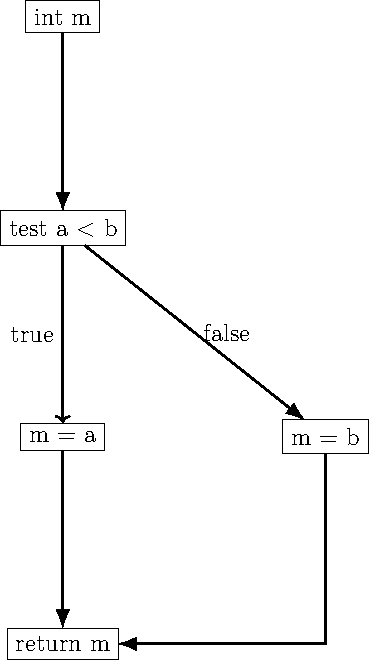
\includegraphics[width=5cm]{img/TP6/cfg_min.pdf} }}%
                \qquad
                \subfloat[\centering ]{{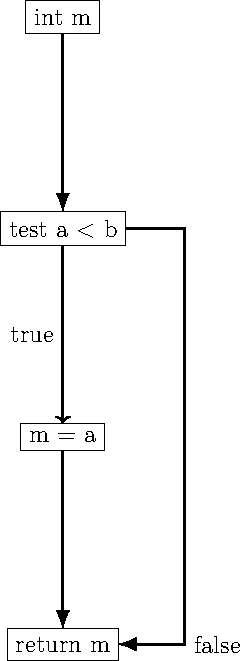
\includegraphics[width=5cm]{img/TP6/cfg_min_alternative.pdf} }}%
                \caption{CFG for min and minAlternative $(a|b|bc)^{*}a$}%
                \label{fig:example}%
            \end{figure}
    \addimg{img/TP6/cfg_squareSum.pdf}{scale=0.5}{CFG for squareSum}{}
    
    Non minimized SSA
    \begin{lstlisting}[language = Java , frame = trBL , firstnumber = last , escapeinside={(*@}{@*)}]
squareSum(n0):
    sum0 = 0
    i0 = 1
    goto loop(n0, sum0, i0)
loop(n1, sum1, i1):
    if i1<=n1 then goto body(n1,sum1,i1) else goto end(n1,sum1,i1)
body(n2, sum2, i2):
    t0 = i2*i2
    sum3 = sum2 + t0
    i3 = i2 + 1
    goto loop(n2, sum3, i3)
end(n3, sum4, i4):
    return sum4
\end{lstlisting}
    Minimized SSA
    \begin{lstlisting}[language = Java , frame = trBL , firstnumber = last , escapeinside={(*@}{@*)}]
squareSum(n0):
    sum0 = 0
    i0 = 1
    goto loop(sum0, i0)
loop(sum1, i1):
    if i1<=n0 then goto body else goto end
body:
    t0 = i1*i1
    sum3 = sum1 + t0
    i3 = i1+1
    goto loop(sum3, i3)
end:
    return sum1
\end{lstlisting}
    Non minimized non-SSA
    \begin{lstlisting}[language = Java , frame = trBL , firstnumber = last , escapeinside={(*@}{@*)}]
squareSum(n):
    sum = 0
    i = 1
    goto loop
loop:
    if i<=n then goto body else goto end
body:
    t = i*i
    sum = sum + t
    i = i +1
    goto loop
end:
    return sum
\end{lstlisting}
    Minimized non-SSA
    \begin{lstlisting}[language = Java , frame = trBL , firstnumber = last , escapeinside={(*@}{@*)}]
squareSum(n0):
    sum0 = 0
    i0 = 1
    sum1 = sum0
    i1 = i0
    goto loop
loop(sum1, i1):
    if i1<=n0 then goto body else goto end
body:
    t0 = i1*i1
    sum3 = sum1 + t0
    i3 = i1+1
    sum1 = sum3
    i1 = i3
    goto loop
end:
    return sum1
\end{lstlisting}

\subsection{Question 3}
    \textbf{Design a simple algorithm that verifies that a function has no missing return statement. The algorithm should also work for complex functions that contain many if-statements, loops, etc.}

    If you represent the start of the function and the end of the function as nodes in the control flow
graph, any path from the start node to the end node must contain a return statement.


\newpage
\section{TP7}
    \subsection{Question 1}
    \textbf{Translate the following function to IR in SSA form and determine the liveness ranges of the variables. Draw the interference graph. Then, allocate registers for an ARM-like CPU and generate machine
code, assuming that the parameter “c” of the function is passed in register r1 (without using the stack. That’s more efficient!) and that the return value of the function should be in register r0.}

    
\begin{table}[H]
    \centering
    \begin{tabular}{|c|c|c|c|c|c|c|c|}
         \hline & t1 & c1 & a1 & t0 & a0 & b0 & c0 \\
         \hline a0 = c0 $\cdot$ 2 &  &  &  &  &  &  & live\\
         \hline b0 = a0 + 1 &  &  &  &  & live &  & live\\
         \hline c1 = c0 + b0 &  &  &  &  & live & live & live \\
         \hline t0 = b0 $\cdot$ 2&  & live &  &  & live & live & \\
         \hline a1 = t0 + a0 &  & live &  & live & live &  & \\
         \hline t1 = c1 + a1 &  & live & live &  &  &  & \\
         \hline return t1& live &  &  &  &  &  & \\
         \hline
    \end{tabular}
    \label{tab:my_label}
\end{table}

    \addimg{img/TP7/1_b.pdf}{}{Interference graph}{}

    \begin{lstlisting}[language = Java , frame = trBL , firstnumber = last , escapeinside={(*@}{@*)}]
pop r0
c0 = r1 (required by the ABI)
a0 = r0
b0 = r2
c1 = r1
t0 = r2
a1 = r0
t1 = r0 (required by the ABI)
\end{lstlisting}


\subsection{Question 2}
    \textbf{In the course, we only saw code generation for functions with parameters and local variables. Now,
let’s look at an example with global variables:}

    \begin{lstlisting}[language = Java , frame = trBL , firstnumber = last , escapeinside={(*@}{@*)}]
int x;
int y[10];

void add(int v) {
    y[x] = v;
    x++;
}
\end{lstlisting}


    \textbf{Translate the above function “add” first to IR code and then to machine code. Assume that the global
variables “x” and “y” start at address 0x10000 and 0x10004, respectively, in main memory.}
    \begin{lstlisting}[language = Java , frame = trBL , firstnumber = last , escapeinside={(*@}{@*)}]
// parameter is v0
t0 = 0x10004
t1 = *t0
 // read value of x
t2 = t1 * 4
 // each array element is four bytes
t3 = 0x10000
t4 = t0 + t3
 // address of y[x]
*t4 = v0
 // store v in y[x]
//-----------
t5 = 0x10004
t6 = *t5
t7 = t6 + 1
*t5 = t7
 // store x+1 in x
\end{lstlisting}

Of course, this code can be optimized. Instead of loading again the variable x in t6, we could just re-use t1.

\subsection{Question 3}
    \textbf{Function calls are expensive because they involve a lot of operations (pushing the arguments on the stack, making backups of registers, jumping to the function, etc.). Many compilers can perform an optimization called function inlining where the code of the called function is directly inserted at the call location, thus avoiding the call. Let’s look at the following example:}

    \begin{lstlisting}[language = Java , frame = trBL , firstnumber = last , escapeinside={(*@}{@*)}]
int f(int v) {
    v = v + 2;
    return v*v;
}
int g(int a, int b) {
    int c = f(a);
    int d = 2*f(a+b);
    return c+d;
}
\end{lstlisting}


    \textbf{Take the role of the compiler and inline the function f at the two places where it is called. Do this inthe IR, not in the source code. Think about a strategy how to handle the variables. By the way, compilers only inline small functions. What could be the reason?}

    \begin{lstlisting}[language = Java , frame = trBL , firstnumber = last , escapeinside={(*@}{@*)}]
// parameters are a0 and b0
v0 = a0
 // calling function f with argument a
v1 = v0 + 2
t0 = v1 * v1
c0 = t0
 // c = f(a)
//-----------
v2 = a0 + b0
 // calling function f with argument a+b
v3 = v2 + 2
t1 = v3 * v3
d0 = 2 * t1
 // d = 2*f(a+b)
//-----------
t2 = c0 + d0
return t2
\end{lstlisting}

Why do compilers only inline small functions? Code size! Inlining increases the number of
instructions in the code and therefore reduces the efficiency of the instruction cache.

\subsection{Question 4}
    \textbf{In most CPUs, integer multiplications are slower than additions or bit shifting. Think about ways to reduce the strength of multiplications, i.e., find ways to avoid the multiplication instruction for arithmetic expressions where one of the operands is a constant, for example }

    \begin{center}
    $x\cdot2$ \\
    $x\cdot3$ \\
    $x\cdot4$ \\
    $x\cdot5$ \\
\end{center}    

    \begin{center}
    $x\cdot2$ = x+x or  x$\verb|<<|$1 \\
    $x\cdot3$ = x+x+x or  x$\verb|<<|$1 + x \\
    $x\cdot4$ = x$\verb|<<|$2 \\
    $x\cdot5$ = x$\verb|<<|$2 + x \\
    x  $\cdot(2^n + 1)$ = (x$\verb|<<|$n) + x
\end{center}
\end{document}
